\chapter{Experiments}\label{chap:experiments}

Experiments were run on a Server with the following specs (Specifics
here\footnote{\url{https://ark.intel.com/content/www/us/en/ark/products/92981/intel-xeon-processor-e5-2630-v4-25m-cache-2-20-ghz.html},
accessed 2019-06-26}):

\begin{table}[ht]
    \ra{1.3}
\begin{tabular}{@{}lr@{}}
    Processor & Intel® Xeon® Processor E5 v4 Family \\
    Number & E5-2630V4 \\ \midrule
    \textbf{Performance} & \\ \midrule
    Number of Cores & 10 \\
    Number of Threads & 20 \\
    Base frequency & 2.2 GHz \\
    Max Turbo frequency & 3.1 GHz \\
    Working Memory (RAM) & 120 GByte \\
\end{tabular}
\end{table}


% Experiments
\todo{The time-resource-measures done}


\begin{figure}[t]
\begin{centering}
    \subfloat[Pairplot over some variables]
    {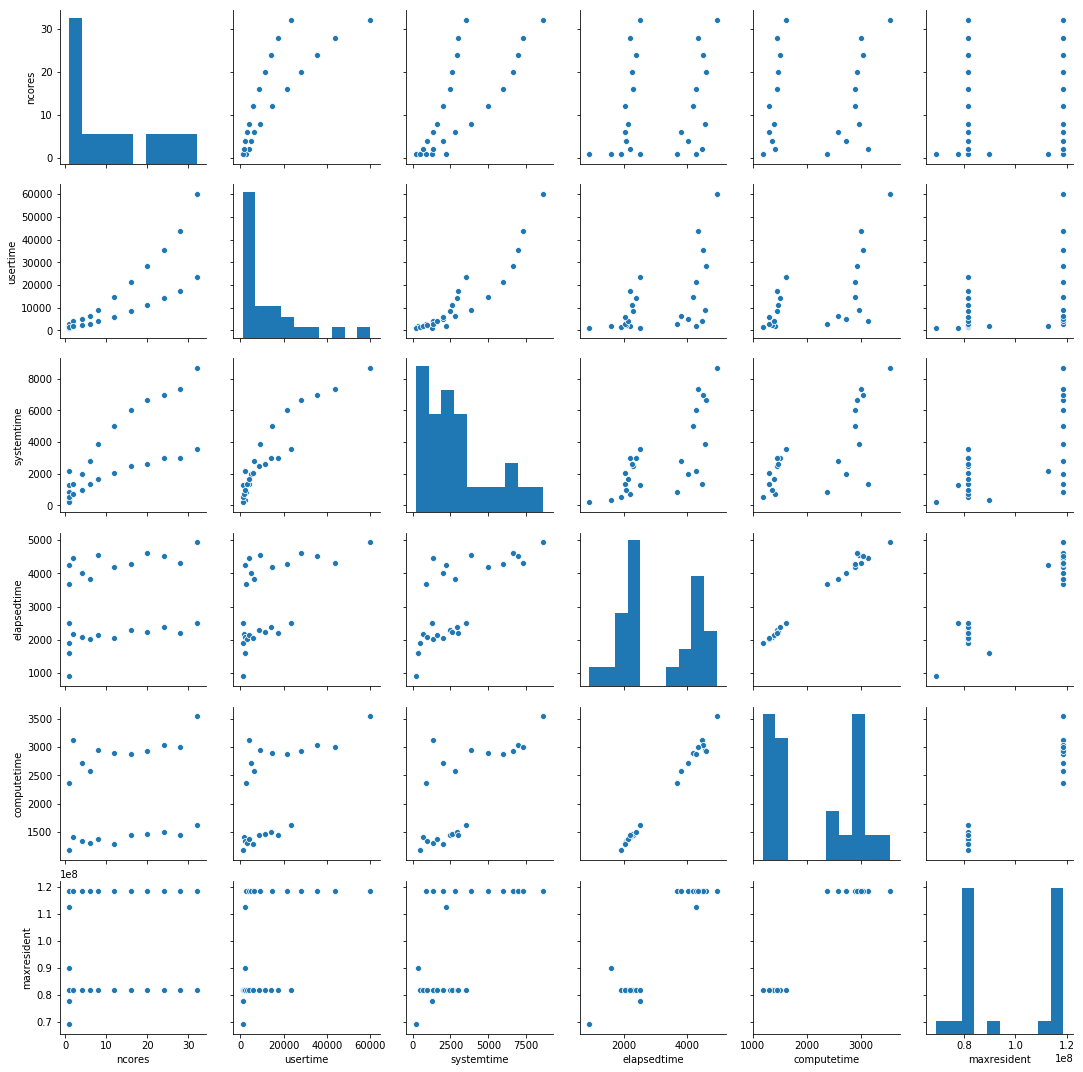
\includegraphics[scale=0.5]{figures/experiments/pairplot.png}}
    \caption[Pairplot]{\textbf{Pairplot over some of the variables ...} moar info here}
    \label{fig:pairplot}
\end{centering}
\end{figure}


\draft{Something is off with my numbers, they show something entirely different from earlier. I'll check that again.}

See \figref{fig:pairplot} (more of that will follow).
